% Компіляція: lualatex -shell-escape main.tex
\documentclass[12pt,a4paper]{article}
\usepackage{fontspec,polyglossia}\setdefaultlanguage{ukrainian}\setmainfont{NewComputerModern10}\setmonofont{Noto Sans Mono}[Scale=.82]
\usepackage{amsmath,booktabs,caption,enumitem,float,fvextra,geometry,graphicx,hyperref,microtype,tikz,titlesec}
\usetikzlibrary{arrows.meta,positioning}
\geometry{left=2cm,right=2cm,top=2cm,bottom=2cm}\setlength{\parindent}{1.25cm}\setlength{\parskip}{0pt}\linespread{1.0}\setlength{\emergencystretch}{3em}
\captionsetup{font=small,labelfont=bf,labelsep=endash}
\titleformat{\section}{\normalfont\fontsize{14}{16}\selectfont\bfseries\centering}{\thesection.}{.6em}{}
\titleformat{\subsection}{\normalfont\fontsize{12}{14}\selectfont\bfseries\centering}{\thesubsection.}{.6em}{}
\begin{document}\pagenumbering{gobble}
\begin{titlepage}
\begin{center}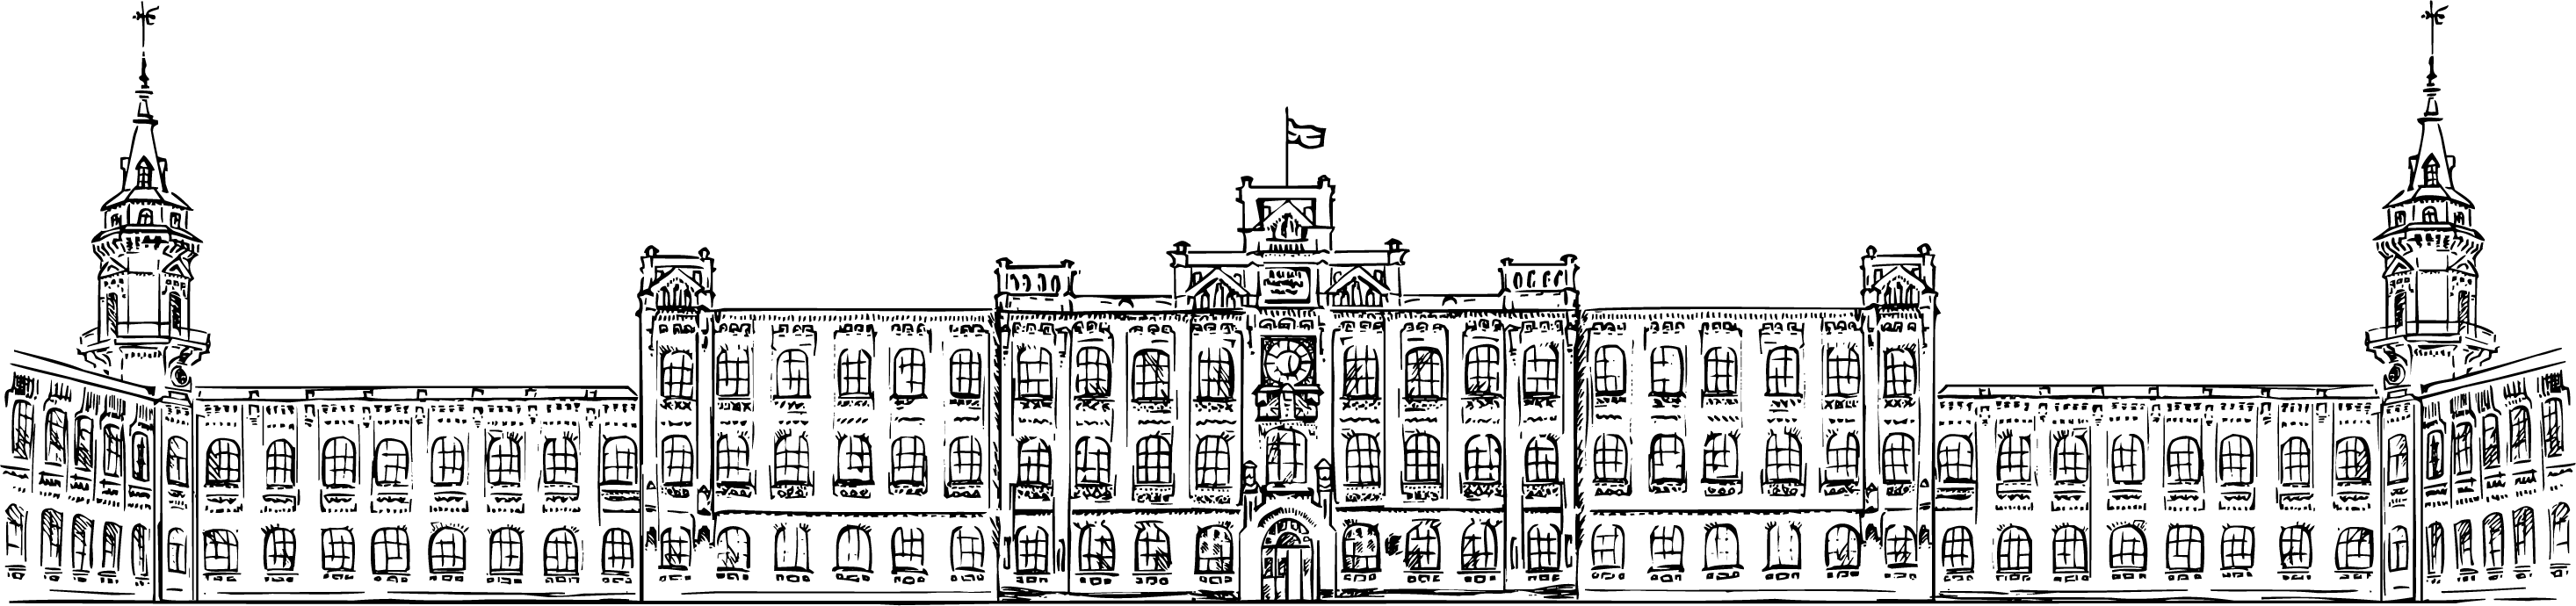
\includegraphics[width=.7\textwidth]{../../../../../../templates/letterhead.png}\end{center}
\begin{center}\large Національний технічний університет України\\«Київський політехнічний інститут імені Ігоря Сікорського»\\[1em]Факультет інформатики та обчислювальної техніки\\Кафедра обчислювальної техніки\end{center}
\vfill\begin{center}\textbf{\LARGE Технології Computer Vision}\\[2em]\textbf{\Large Лабораторна робота №9}\\[.7em]«Проєктний практикум: синтез реалістичних 3D-об'єктів»\end{center}
\vfill\begin{flushright}\begin{minipage}{.48\textwidth}Виконав: студент 3 курсу ФІОТ,\\групи ІО-41\\\textit{Давидчук А. М.}\\Залікова книжка № 4106\\[1em]Перевірив: \textit{Баран Д. Р.}\end{minipage}\end{flushright}
\vfill\begin{center}Київ --- 2026\end{center}\end{titlepage}
\pagenumbering{arabic}

\section{Тема та мета роботи}
\noindent\textbf{Тема:} синтез динамічної тривимірної сцени засобами 3D Computer Vision.

\medskip\noindent\textbf{Мета:} дослідити методологію створення доповненої реальності та взаємодію об'єкта, освітлення й спостерігача.

\section{Завдання роботи}
Основне завдання методички --- створити Python-скрипт реалістичної візуалізації графічної сцени відповідно до взаємодії її об'єктів. Виконується варіант 9: для формування модельного Dataset із метою подальшого навчання нейромережі для розпізнавання об'єктів створити динамічну модель руху бронетехніки.

Сцена містить бронемашину, дорогу, рельєф, розмітку та статичні об'єкти. Корпус рухається за траєкторією, башта повертається незалежно, а камера плавно змінює азимут. Кожен кадр зберігається разом із координатами й кутом башти.

\section{Математична модель}
Положення центра машини у кадрі $t$, $t\in[0,1]$:
\begin{equation}x(t)=-6{,}2+12{,}4t,\qquad y(t)=0{,}65\sin(2\pi t).\end{equation}
Кут башти:
\begin{equation}\theta(t)=0{,}35\sin(4\pi t).\end{equation}
Кінець ствола довжини $L=2{,}7$ визначається як
\begin{equation}p_{gun}=p_{turret}+[L\cos\theta,L\sin\theta,0]^T.\end{equation}
Прямокутні частини техніки задаються вісьмома вершинами паралелепіпеда. Кожна грань проєктується перспективною камерою на площину кадру. Підпис набору даних:
\begin{equation}y_i=(i,x_i,y_i,\theta_i,\texttt{armored\_vehicle}).\end{equation}

\section{Архітектура рішення}
\begin{figure}[H]\centering
\begin{tikzpicture}[node distance=.65cm,block/.style={draw,rounded corners,align=center,minimum width=2.8cm,minimum height=.8cm,fill=blue!7},arrow/.style={-{Latex},thick}]
\node[block](a){3D-моделі\\сцени};\node[block,right=of a](b){Траєкторія\\і поворот башти};\node[block,right=of b](c){Перспективна\\камера};
\node[block,below=of c](d){Рендеринг\\42 кадрів};\node[block,left=of d](e){Dataset JPEG\\+ CSV-мітки};\node[block,left=of e](f){GIF та\\контрольна мозаїка};
\draw[arrow](a)--(b)--(c)--(d)--(e)--(f);
\end{tikzpicture}\caption{Блок-схема синтезу динамічної сцени}
\end{figure}

\section{Результати}
Сформовано 42 кадри з частотою 12 кадрів/с, тобто 3,5 с анімації. Кадри знаходяться у каталозі \texttt{results/dataset}, а мітки --- у \texttt{dataset\_labels.csv}.
\begin{figure}[H]\centering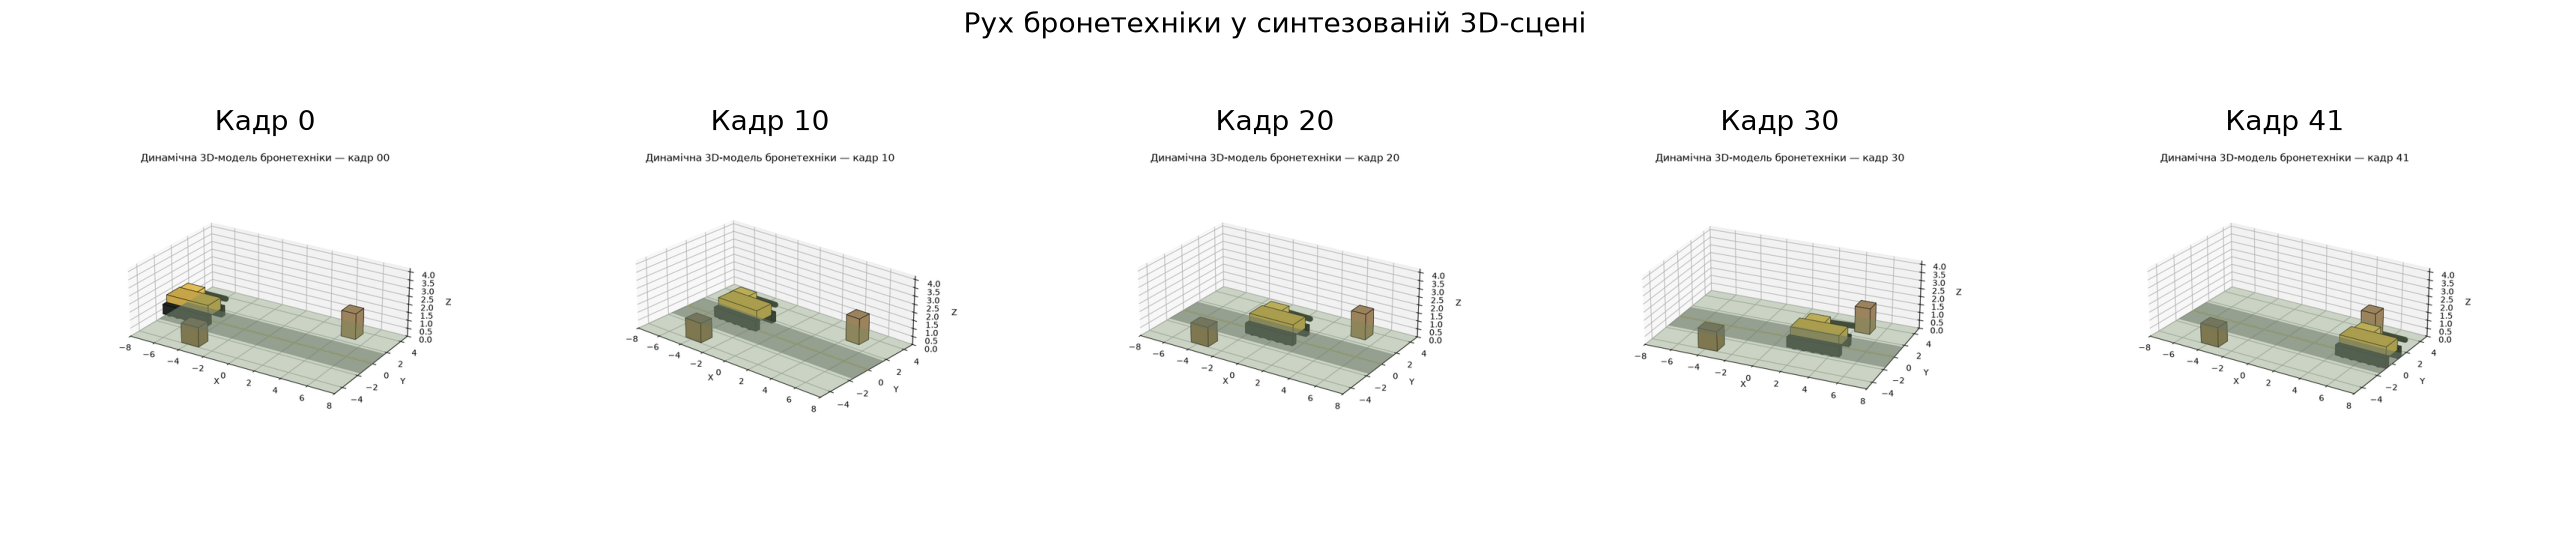
\includegraphics[width=.98\textwidth]{../results/scene_montage.png}\caption{Ключові положення бронетехніки у 3D-сцені}\end{figure}
\begin{figure}[H]\centering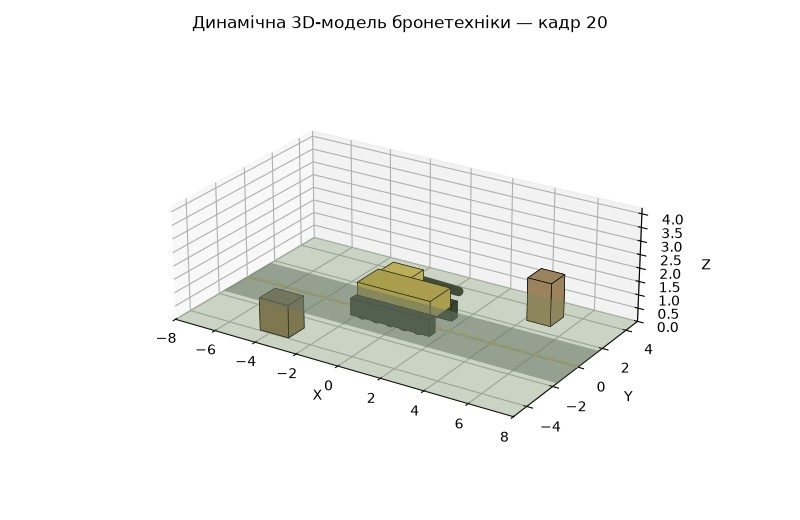
\includegraphics[width=.88\textwidth]{../results/dataset/frame_020.jpg}\caption{Окремий кадр синтезованого набору даних}\end{figure}
\begin{table}[H]\centering\caption{Характеристики сформованого Dataset}
\begin{tabular}{lr}\toprule Показник&Значення\\\midrule Кількість кадрів&42\\Розмір кадру&800$\times$520\\Клас&armored\_vehicle\\Параметри пози&$x,y,\theta$\\Тривалість GIF&3,50 с\\\bottomrule\end{tabular}
\end{table}
На послідовності видно переміщення корпусу вздовж дороги, поперечне відхилення, незалежний поворот башти та зміну точки спостереження. Статичні об'єкти задають просторовий контекст і дозволяють оцінити перспективу.

\section{Структура проєкту}
\begin{verbatim}
lab9/
|-- src/main.py
|-- results/
|   |-- dataset/frame_000.jpg ... frame_041.jpg
|   |-- dataset_labels.csv
|   |-- armored_vehicle.gif
|   `-- scene_montage.png
|-- requirements.txt
`-- docs/main.tex, main.pdf
\end{verbatim}

\section{Висновки}
Виконано варіант 9: створено динамічну 3D-модель руху бронетехніки та сформовано підписаний модельний Dataset. Реалізація враховує композицію сцени, рух, незалежну орієнтацію башти й перспективу спостерігача. Отримані кадри придатні для демонстрації та як початкові синтетичні дані; для навчання промислової моделі потрібні варіації текстур, освітлення, погоди та ракурсів.

\section{Лістинг програми}
\VerbatimInput[fontsize=\small,numbers=left,breaklines=true,frame=single]{../src/main.py}
\end{document}
